% Created by tikzDevice version 0.6.1 on 2016-02-24 23:26:46
% !TEX encoding = UTF-8 Unicode
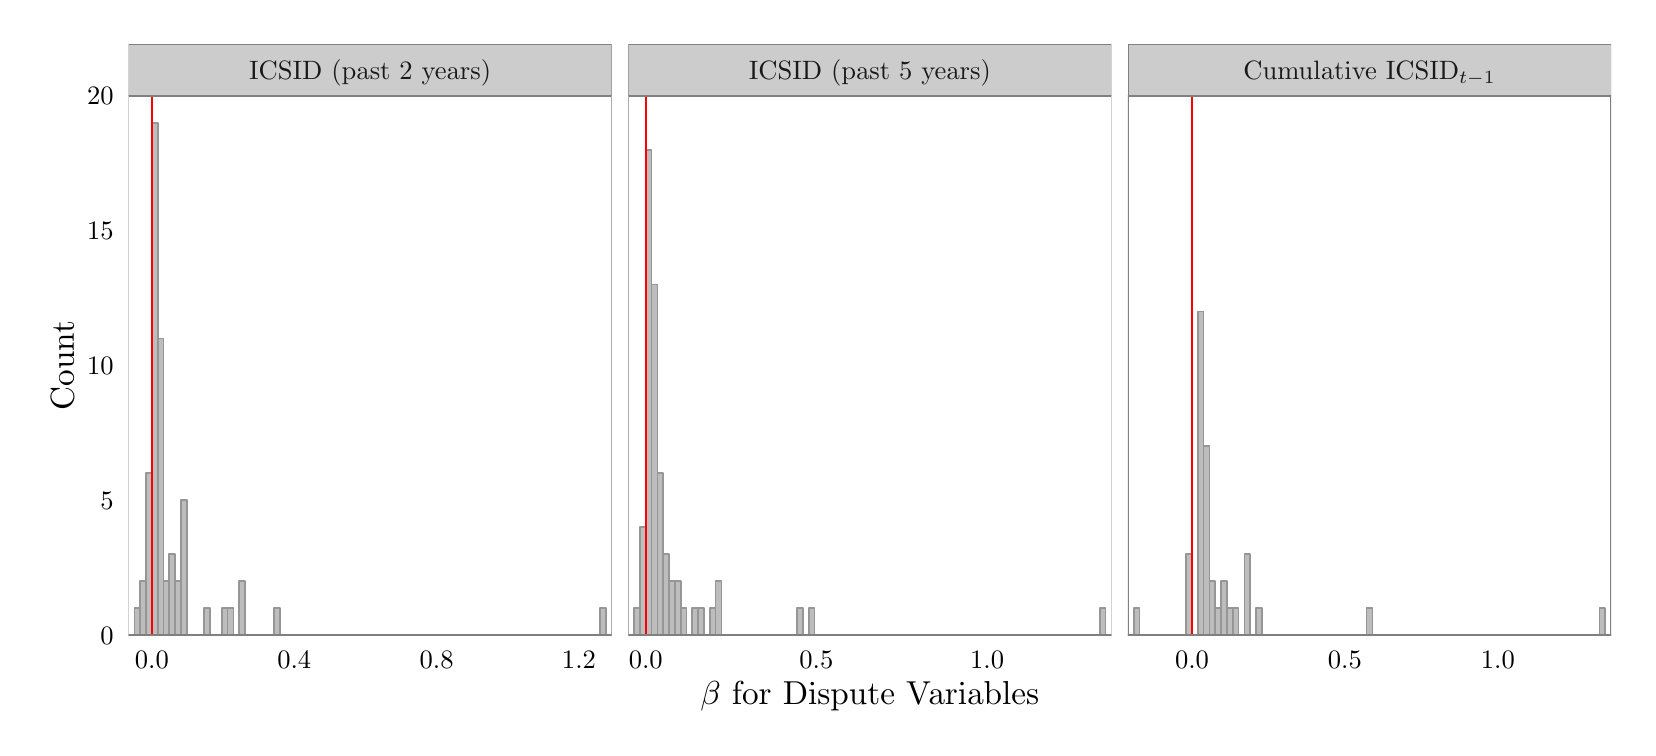
\begin{tikzpicture}[x=1pt,y=1pt]
\definecolor[named]{drawColor}{rgb}{0.00,0.00,0.00}
\definecolor[named]{fillColor}{rgb}{1.00,1.00,1.00}
\fill[color=fillColor,] (0,0) rectangle (578.16,252.94);
\begin{scope}
\path[clip] (  0.00,  0.00) rectangle (578.16,252.94);
\end{scope}
\begin{scope}
\path[clip] (  0.00,  0.00) rectangle (578.16,252.94);
\end{scope}
\begin{scope}
\path[clip] (  0.00,  0.00) rectangle (578.16,252.94);
\end{scope}
\begin{scope}
\path[clip] (  0.00,  0.00) rectangle (578.16,252.94);
\end{scope}
\begin{scope}
\path[clip] (  0.00,  0.00) rectangle (578.16,252.94);
\end{scope}
\begin{scope}
\path[clip] (  0.00,  0.00) rectangle (578.16,252.94);
\end{scope}
\begin{scope}
\path[clip] (  0.00,  0.00) rectangle (578.16,252.94);
\end{scope}
\begin{scope}
\path[clip] (  0.00,  0.00) rectangle (578.16,252.94);
\end{scope}
\begin{scope}
\path[clip] (  0.00,  0.00) rectangle (578.16,252.94);
\end{scope}
\begin{scope}
\path[clip] (  0.00,  0.00) rectangle (578.16,252.94);
\end{scope}
\begin{scope}
\path[clip] (  0.00,  0.00) rectangle (578.16,252.94);
\end{scope}
\begin{scope}
\path[clip] (  0.00,  0.00) rectangle (578.16,252.94);
\end{scope}
\begin{scope}
\path[clip] (  0.00,  0.00) rectangle (578.16,252.94);
\end{scope}
\begin{scope}
\path[clip] (  0.00,  0.00) rectangle (578.16,252.94);
\definecolor[named]{drawColor}{rgb}{1.00,1.00,1.00}
\definecolor[named]{fillColor}{rgb}{1.00,1.00,1.00}

\draw[color=drawColor,line width= 0.6pt,line cap=round,line join=round,fill=fillColor,] (  0.00,  0.00) rectangle (578.16,252.95);
\end{scope}
\begin{scope}
\path[clip] (  0.00,  0.00) rectangle (578.16,252.94);
\end{scope}
\begin{scope}
\path[clip] ( 36.46, 33.48) rectangle (211.03,228.33);
\definecolor[named]{fillColor}{rgb}{1.00,1.00,1.00}

\draw[fill=fillColor,draw opacity=0.00,] ( 36.46, 33.48) rectangle (211.03,228.33);
\definecolor[named]{drawColor}{rgb}{0.59,0.59,0.59}
\definecolor[named]{fillColor}{rgb}{0.74,0.74,0.74}

\draw[color=drawColor,line width= 0.6pt,line join=round,fill=fillColor,] ( 36.46, 33.48) rectangle ( 38.57, 33.48);

\draw[color=drawColor,line width= 0.6pt,line join=round,fill=fillColor,] ( 38.57, 33.48) rectangle ( 40.67, 43.22);

\draw[color=drawColor,line width= 0.6pt,line join=round,fill=fillColor,] ( 40.67, 33.48) rectangle ( 42.77, 52.96);

\draw[color=drawColor,line width= 0.6pt,line join=round,fill=fillColor,] ( 42.77, 33.48) rectangle ( 44.88, 91.93);

\draw[color=drawColor,line width= 0.6pt,line join=round,fill=fillColor,] ( 44.88, 33.48) rectangle ( 46.98,218.59);

\draw[color=drawColor,line width= 0.6pt,line join=round,fill=fillColor,] ( 46.98, 33.48) rectangle ( 49.08,140.65);

\draw[color=drawColor,line width= 0.6pt,line join=round,fill=fillColor,] ( 49.08, 33.48) rectangle ( 51.18, 52.96);

\draw[color=drawColor,line width= 0.6pt,line join=round,fill=fillColor,] ( 51.18, 33.48) rectangle ( 53.29, 62.70);

\draw[color=drawColor,line width= 0.6pt,line join=round,fill=fillColor,] ( 53.29, 33.48) rectangle ( 55.39, 52.96);

\draw[color=drawColor,line width= 0.6pt,line join=round,fill=fillColor,] ( 55.39, 33.48) rectangle ( 57.49, 82.19);

\draw[color=drawColor,line width= 0.6pt,line join=round,fill=fillColor,] ( 57.49, 33.48) rectangle ( 59.60, 33.48);

\draw[color=drawColor,line width= 0.6pt,line join=round,fill=fillColor,] ( 59.60, 33.48) rectangle ( 61.70, 33.48);

\draw[color=drawColor,line width= 0.6pt,line join=round,fill=fillColor,] ( 61.70, 33.48) rectangle ( 63.80, 33.48);

\draw[color=drawColor,line width= 0.6pt,line join=round,fill=fillColor,] ( 63.80, 33.48) rectangle ( 65.91, 43.22);

\draw[color=drawColor,line width= 0.6pt,line join=round,fill=fillColor,] ( 65.91, 33.48) rectangle ( 68.01, 33.48);

\draw[color=drawColor,line width= 0.6pt,line join=round,fill=fillColor,] ( 68.01, 33.48) rectangle ( 70.11, 33.48);

\draw[color=drawColor,line width= 0.6pt,line join=round,fill=fillColor,] ( 70.11, 33.48) rectangle ( 72.22, 43.22);

\draw[color=drawColor,line width= 0.6pt,line join=round,fill=fillColor,] ( 72.22, 33.48) rectangle ( 74.32, 43.22);

\draw[color=drawColor,line width= 0.6pt,line join=round,fill=fillColor,] ( 74.32, 33.48) rectangle ( 76.42, 33.48);

\draw[color=drawColor,line width= 0.6pt,line join=round,fill=fillColor,] ( 76.42, 33.48) rectangle ( 78.53, 52.96);

\draw[color=drawColor,line width= 0.6pt,line join=round,fill=fillColor,] ( 78.53, 33.48) rectangle ( 80.63, 33.48);

\draw[color=drawColor,line width= 0.6pt,line join=round,fill=fillColor,] ( 80.63, 33.48) rectangle ( 82.73, 33.48);

\draw[color=drawColor,line width= 0.6pt,line join=round,fill=fillColor,] ( 82.73, 33.48) rectangle ( 84.84, 33.48);

\draw[color=drawColor,line width= 0.6pt,line join=round,fill=fillColor,] ( 84.84, 33.48) rectangle ( 86.94, 33.48);

\draw[color=drawColor,line width= 0.6pt,line join=round,fill=fillColor,] ( 86.94, 33.48) rectangle ( 89.04, 33.48);

\draw[color=drawColor,line width= 0.6pt,line join=round,fill=fillColor,] ( 89.04, 33.48) rectangle ( 91.15, 43.22);

\draw[color=drawColor,line width= 0.6pt,line join=round,fill=fillColor,] ( 91.15, 33.48) rectangle ( 93.25, 33.48);

\draw[color=drawColor,line width= 0.6pt,line join=round,fill=fillColor,] ( 93.25, 33.48) rectangle ( 95.35, 33.48);

\draw[color=drawColor,line width= 0.6pt,line join=round,fill=fillColor,] ( 95.35, 33.48) rectangle ( 97.46, 33.48);

\draw[color=drawColor,line width= 0.6pt,line join=round,fill=fillColor,] ( 97.46, 33.48) rectangle ( 99.56, 33.48);

\draw[color=drawColor,line width= 0.6pt,line join=round,fill=fillColor,] ( 99.56, 33.48) rectangle (101.66, 33.48);

\draw[color=drawColor,line width= 0.6pt,line join=round,fill=fillColor,] (101.66, 33.48) rectangle (103.76, 33.48);

\draw[color=drawColor,line width= 0.6pt,line join=round,fill=fillColor,] (103.76, 33.48) rectangle (105.87, 33.48);

\draw[color=drawColor,line width= 0.6pt,line join=round,fill=fillColor,] (105.87, 33.48) rectangle (107.97, 33.48);

\draw[color=drawColor,line width= 0.6pt,line join=round,fill=fillColor,] (107.97, 33.48) rectangle (110.07, 33.48);

\draw[color=drawColor,line width= 0.6pt,line join=round,fill=fillColor,] (110.07, 33.48) rectangle (112.18, 33.48);

\draw[color=drawColor,line width= 0.6pt,line join=round,fill=fillColor,] (112.18, 33.48) rectangle (114.28, 33.48);

\draw[color=drawColor,line width= 0.6pt,line join=round,fill=fillColor,] (114.28, 33.48) rectangle (116.38, 33.48);

\draw[color=drawColor,line width= 0.6pt,line join=round,fill=fillColor,] (116.38, 33.48) rectangle (118.49, 33.48);

\draw[color=drawColor,line width= 0.6pt,line join=round,fill=fillColor,] (118.49, 33.48) rectangle (120.59, 33.48);

\draw[color=drawColor,line width= 0.6pt,line join=round,fill=fillColor,] (120.59, 33.48) rectangle (122.69, 33.48);

\draw[color=drawColor,line width= 0.6pt,line join=round,fill=fillColor,] (122.69, 33.48) rectangle (124.80, 33.48);

\draw[color=drawColor,line width= 0.6pt,line join=round,fill=fillColor,] (124.80, 33.48) rectangle (126.90, 33.48);

\draw[color=drawColor,line width= 0.6pt,line join=round,fill=fillColor,] (126.90, 33.48) rectangle (129.00, 33.48);

\draw[color=drawColor,line width= 0.6pt,line join=round,fill=fillColor,] (129.00, 33.48) rectangle (131.11, 33.48);

\draw[color=drawColor,line width= 0.6pt,line join=round,fill=fillColor,] (131.11, 33.48) rectangle (133.21, 33.48);

\draw[color=drawColor,line width= 0.6pt,line join=round,fill=fillColor,] (133.21, 33.48) rectangle (135.31, 33.48);

\draw[color=drawColor,line width= 0.6pt,line join=round,fill=fillColor,] (135.31, 33.48) rectangle (137.42, 33.48);

\draw[color=drawColor,line width= 0.6pt,line join=round,fill=fillColor,] (137.42, 33.48) rectangle (139.52, 33.48);

\draw[color=drawColor,line width= 0.6pt,line join=round,fill=fillColor,] (139.52, 33.48) rectangle (141.62, 33.48);

\draw[color=drawColor,line width= 0.6pt,line join=round,fill=fillColor,] (141.62, 33.48) rectangle (143.73, 33.48);

\draw[color=drawColor,line width= 0.6pt,line join=round,fill=fillColor,] (143.73, 33.48) rectangle (145.83, 33.48);

\draw[color=drawColor,line width= 0.6pt,line join=round,fill=fillColor,] (145.83, 33.48) rectangle (147.93, 33.48);

\draw[color=drawColor,line width= 0.6pt,line join=round,fill=fillColor,] (147.93, 33.48) rectangle (150.04, 33.48);

\draw[color=drawColor,line width= 0.6pt,line join=round,fill=fillColor,] (150.04, 33.48) rectangle (152.14, 33.48);

\draw[color=drawColor,line width= 0.6pt,line join=round,fill=fillColor,] (152.14, 33.48) rectangle (154.24, 33.48);

\draw[color=drawColor,line width= 0.6pt,line join=round,fill=fillColor,] (154.24, 33.48) rectangle (156.34, 33.48);

\draw[color=drawColor,line width= 0.6pt,line join=round,fill=fillColor,] (156.34, 33.48) rectangle (158.45, 33.48);

\draw[color=drawColor,line width= 0.6pt,line join=round,fill=fillColor,] (158.45, 33.48) rectangle (160.55, 33.48);

\draw[color=drawColor,line width= 0.6pt,line join=round,fill=fillColor,] (160.55, 33.48) rectangle (162.65, 33.48);

\draw[color=drawColor,line width= 0.6pt,line join=round,fill=fillColor,] (162.65, 33.48) rectangle (164.76, 33.48);

\draw[color=drawColor,line width= 0.6pt,line join=round,fill=fillColor,] (164.76, 33.48) rectangle (166.86, 33.48);

\draw[color=drawColor,line width= 0.6pt,line join=round,fill=fillColor,] (166.86, 33.48) rectangle (168.96, 33.48);

\draw[color=drawColor,line width= 0.6pt,line join=round,fill=fillColor,] (168.96, 33.48) rectangle (171.07, 33.48);

\draw[color=drawColor,line width= 0.6pt,line join=round,fill=fillColor,] (171.07, 33.48) rectangle (173.17, 33.48);

\draw[color=drawColor,line width= 0.6pt,line join=round,fill=fillColor,] (173.17, 33.48) rectangle (175.27, 33.48);

\draw[color=drawColor,line width= 0.6pt,line join=round,fill=fillColor,] (175.27, 33.48) rectangle (177.38, 33.48);

\draw[color=drawColor,line width= 0.6pt,line join=round,fill=fillColor,] (177.38, 33.48) rectangle (179.48, 33.48);

\draw[color=drawColor,line width= 0.6pt,line join=round,fill=fillColor,] (179.48, 33.48) rectangle (181.58, 33.48);

\draw[color=drawColor,line width= 0.6pt,line join=round,fill=fillColor,] (181.58, 33.48) rectangle (183.69, 33.48);

\draw[color=drawColor,line width= 0.6pt,line join=round,fill=fillColor,] (183.69, 33.48) rectangle (185.79, 33.48);

\draw[color=drawColor,line width= 0.6pt,line join=round,fill=fillColor,] (185.79, 33.48) rectangle (187.89, 33.48);

\draw[color=drawColor,line width= 0.6pt,line join=round,fill=fillColor,] (187.89, 33.48) rectangle (190.00, 33.48);

\draw[color=drawColor,line width= 0.6pt,line join=round,fill=fillColor,] (190.00, 33.48) rectangle (192.10, 33.48);

\draw[color=drawColor,line width= 0.6pt,line join=round,fill=fillColor,] (192.10, 33.48) rectangle (194.20, 33.48);

\draw[color=drawColor,line width= 0.6pt,line join=round,fill=fillColor,] (194.20, 33.48) rectangle (196.31, 33.48);

\draw[color=drawColor,line width= 0.6pt,line join=round,fill=fillColor,] (196.31, 33.48) rectangle (198.41, 33.48);

\draw[color=drawColor,line width= 0.6pt,line join=round,fill=fillColor,] (198.41, 33.48) rectangle (200.51, 33.48);

\draw[color=drawColor,line width= 0.6pt,line join=round,fill=fillColor,] (200.51, 33.48) rectangle (202.62, 33.48);

\draw[color=drawColor,line width= 0.6pt,line join=round,fill=fillColor,] (202.62, 33.48) rectangle (204.72, 33.48);

\draw[color=drawColor,line width= 0.6pt,line join=round,fill=fillColor,] (204.72, 33.48) rectangle (206.82, 33.48);

\draw[color=drawColor,line width= 0.6pt,line join=round,fill=fillColor,] (206.82, 33.48) rectangle (208.93, 43.22);

\draw[color=drawColor,line width= 0.6pt,line join=round,fill=fillColor,] (208.93, 33.48) rectangle (211.03, 33.48);
\definecolor[named]{drawColor}{rgb}{1.00,0.00,0.00}
\definecolor[named]{fillColor}{rgb}{1.00,0.00,0.00}

\draw[color=drawColor,line width= 0.6pt,line join=round,fill=fillColor,] ( 44.88, 33.48) -- ( 44.88,228.33);
\definecolor[named]{drawColor}{rgb}{0.50,0.50,0.50}

\draw[color=drawColor,line width= 0.6pt,line cap=round,line join=round,fill opacity=0.00,] ( 36.46, 33.48) rectangle (211.03,228.33);
\end{scope}
\begin{scope}
\path[clip] (  0.00,  0.00) rectangle (578.16,252.94);
\end{scope}
\begin{scope}
\path[clip] (217.03, 33.48) rectangle (391.59,228.33);
\definecolor[named]{fillColor}{rgb}{1.00,1.00,1.00}

\draw[fill=fillColor,draw opacity=0.00,] (217.03, 33.48) rectangle (391.59,228.33);
\definecolor[named]{drawColor}{rgb}{0.59,0.59,0.59}
\definecolor[named]{fillColor}{rgb}{0.74,0.74,0.74}

\draw[color=drawColor,line width= 0.6pt,line join=round,fill=fillColor,] (217.03, 33.48) rectangle (219.13, 33.48);

\draw[color=drawColor,line width= 0.6pt,line join=round,fill=fillColor,] (219.13, 33.48) rectangle (221.23, 43.22);

\draw[color=drawColor,line width= 0.6pt,line join=round,fill=fillColor,] (221.23, 33.48) rectangle (223.34, 72.45);

\draw[color=drawColor,line width= 0.6pt,line join=round,fill=fillColor,] (223.34, 33.48) rectangle (225.44,208.85);

\draw[color=drawColor,line width= 0.6pt,line join=round,fill=fillColor,] (225.44, 33.48) rectangle (227.54,160.13);

\draw[color=drawColor,line width= 0.6pt,line join=round,fill=fillColor,] (227.54, 33.48) rectangle (229.65, 91.93);

\draw[color=drawColor,line width= 0.6pt,line join=round,fill=fillColor,] (229.65, 33.48) rectangle (231.75, 62.70);

\draw[color=drawColor,line width= 0.6pt,line join=round,fill=fillColor,] (231.75, 33.48) rectangle (233.85, 52.96);

\draw[color=drawColor,line width= 0.6pt,line join=round,fill=fillColor,] (233.85, 33.48) rectangle (235.96, 52.96);

\draw[color=drawColor,line width= 0.6pt,line join=round,fill=fillColor,] (235.96, 33.48) rectangle (238.06, 43.22);

\draw[color=drawColor,line width= 0.6pt,line join=round,fill=fillColor,] (238.06, 33.48) rectangle (240.16, 33.48);

\draw[color=drawColor,line width= 0.6pt,line join=round,fill=fillColor,] (240.16, 33.48) rectangle (242.27, 43.22);

\draw[color=drawColor,line width= 0.6pt,line join=round,fill=fillColor,] (242.27, 33.48) rectangle (244.37, 43.22);

\draw[color=drawColor,line width= 0.6pt,line join=round,fill=fillColor,] (244.37, 33.48) rectangle (246.47, 33.48);

\draw[color=drawColor,line width= 0.6pt,line join=round,fill=fillColor,] (246.47, 33.48) rectangle (248.58, 43.22);

\draw[color=drawColor,line width= 0.6pt,line join=round,fill=fillColor,] (248.58, 33.48) rectangle (250.68, 52.96);

\draw[color=drawColor,line width= 0.6pt,line join=round,fill=fillColor,] (250.68, 33.48) rectangle (252.78, 33.48);

\draw[color=drawColor,line width= 0.6pt,line join=round,fill=fillColor,] (252.78, 33.48) rectangle (254.89, 33.48);

\draw[color=drawColor,line width= 0.6pt,line join=round,fill=fillColor,] (254.89, 33.48) rectangle (256.99, 33.48);

\draw[color=drawColor,line width= 0.6pt,line join=round,fill=fillColor,] (256.99, 33.48) rectangle (259.09, 33.48);

\draw[color=drawColor,line width= 0.6pt,line join=round,fill=fillColor,] (259.09, 33.48) rectangle (261.20, 33.48);

\draw[color=drawColor,line width= 0.6pt,line join=round,fill=fillColor,] (261.20, 33.48) rectangle (263.30, 33.48);

\draw[color=drawColor,line width= 0.6pt,line join=round,fill=fillColor,] (263.30, 33.48) rectangle (265.40, 33.48);

\draw[color=drawColor,line width= 0.6pt,line join=round,fill=fillColor,] (265.40, 33.48) rectangle (267.51, 33.48);

\draw[color=drawColor,line width= 0.6pt,line join=round,fill=fillColor,] (267.51, 33.48) rectangle (269.61, 33.48);

\draw[color=drawColor,line width= 0.6pt,line join=round,fill=fillColor,] (269.61, 33.48) rectangle (271.71, 33.48);

\draw[color=drawColor,line width= 0.6pt,line join=round,fill=fillColor,] (271.71, 33.48) rectangle (273.81, 33.48);

\draw[color=drawColor,line width= 0.6pt,line join=round,fill=fillColor,] (273.81, 33.48) rectangle (275.92, 33.48);

\draw[color=drawColor,line width= 0.6pt,line join=round,fill=fillColor,] (275.92, 33.48) rectangle (278.02, 33.48);

\draw[color=drawColor,line width= 0.6pt,line join=round,fill=fillColor,] (278.02, 33.48) rectangle (280.12, 43.22);

\draw[color=drawColor,line width= 0.6pt,line join=round,fill=fillColor,] (280.12, 33.48) rectangle (282.23, 33.48);

\draw[color=drawColor,line width= 0.6pt,line join=round,fill=fillColor,] (282.23, 33.48) rectangle (284.33, 43.22);

\draw[color=drawColor,line width= 0.6pt,line join=round,fill=fillColor,] (284.33, 33.48) rectangle (286.43, 33.48);

\draw[color=drawColor,line width= 0.6pt,line join=round,fill=fillColor,] (286.43, 33.48) rectangle (288.54, 33.48);

\draw[color=drawColor,line width= 0.6pt,line join=round,fill=fillColor,] (288.54, 33.48) rectangle (290.64, 33.48);

\draw[color=drawColor,line width= 0.6pt,line join=round,fill=fillColor,] (290.64, 33.48) rectangle (292.74, 33.48);

\draw[color=drawColor,line width= 0.6pt,line join=round,fill=fillColor,] (292.74, 33.48) rectangle (294.85, 33.48);

\draw[color=drawColor,line width= 0.6pt,line join=round,fill=fillColor,] (294.85, 33.48) rectangle (296.95, 33.48);

\draw[color=drawColor,line width= 0.6pt,line join=round,fill=fillColor,] (296.95, 33.48) rectangle (299.05, 33.48);

\draw[color=drawColor,line width= 0.6pt,line join=round,fill=fillColor,] (299.05, 33.48) rectangle (301.16, 33.48);

\draw[color=drawColor,line width= 0.6pt,line join=round,fill=fillColor,] (301.16, 33.48) rectangle (303.26, 33.48);

\draw[color=drawColor,line width= 0.6pt,line join=round,fill=fillColor,] (303.26, 33.48) rectangle (305.36, 33.48);

\draw[color=drawColor,line width= 0.6pt,line join=round,fill=fillColor,] (305.36, 33.48) rectangle (307.47, 33.48);

\draw[color=drawColor,line width= 0.6pt,line join=round,fill=fillColor,] (307.47, 33.48) rectangle (309.57, 33.48);

\draw[color=drawColor,line width= 0.6pt,line join=round,fill=fillColor,] (309.57, 33.48) rectangle (311.67, 33.48);

\draw[color=drawColor,line width= 0.6pt,line join=round,fill=fillColor,] (311.67, 33.48) rectangle (313.78, 33.48);

\draw[color=drawColor,line width= 0.6pt,line join=round,fill=fillColor,] (313.78, 33.48) rectangle (315.88, 33.48);

\draw[color=drawColor,line width= 0.6pt,line join=round,fill=fillColor,] (315.88, 33.48) rectangle (317.98, 33.48);

\draw[color=drawColor,line width= 0.6pt,line join=round,fill=fillColor,] (317.98, 33.48) rectangle (320.09, 33.48);

\draw[color=drawColor,line width= 0.6pt,line join=round,fill=fillColor,] (320.09, 33.48) rectangle (322.19, 33.48);

\draw[color=drawColor,line width= 0.6pt,line join=round,fill=fillColor,] (322.19, 33.48) rectangle (324.29, 33.48);

\draw[color=drawColor,line width= 0.6pt,line join=round,fill=fillColor,] (324.29, 33.48) rectangle (326.39, 33.48);

\draw[color=drawColor,line width= 0.6pt,line join=round,fill=fillColor,] (326.39, 33.48) rectangle (328.50, 33.48);

\draw[color=drawColor,line width= 0.6pt,line join=round,fill=fillColor,] (328.50, 33.48) rectangle (330.60, 33.48);

\draw[color=drawColor,line width= 0.6pt,line join=round,fill=fillColor,] (330.60, 33.48) rectangle (332.70, 33.48);

\draw[color=drawColor,line width= 0.6pt,line join=round,fill=fillColor,] (332.70, 33.48) rectangle (334.81, 33.48);

\draw[color=drawColor,line width= 0.6pt,line join=round,fill=fillColor,] (334.81, 33.48) rectangle (336.91, 33.48);

\draw[color=drawColor,line width= 0.6pt,line join=round,fill=fillColor,] (336.91, 33.48) rectangle (339.01, 33.48);

\draw[color=drawColor,line width= 0.6pt,line join=round,fill=fillColor,] (339.01, 33.48) rectangle (341.12, 33.48);

\draw[color=drawColor,line width= 0.6pt,line join=round,fill=fillColor,] (341.12, 33.48) rectangle (343.22, 33.48);

\draw[color=drawColor,line width= 0.6pt,line join=round,fill=fillColor,] (343.22, 33.48) rectangle (345.32, 33.48);

\draw[color=drawColor,line width= 0.6pt,line join=round,fill=fillColor,] (345.32, 33.48) rectangle (347.43, 33.48);

\draw[color=drawColor,line width= 0.6pt,line join=round,fill=fillColor,] (347.43, 33.48) rectangle (349.53, 33.48);

\draw[color=drawColor,line width= 0.6pt,line join=round,fill=fillColor,] (349.53, 33.48) rectangle (351.63, 33.48);

\draw[color=drawColor,line width= 0.6pt,line join=round,fill=fillColor,] (351.63, 33.48) rectangle (353.74, 33.48);

\draw[color=drawColor,line width= 0.6pt,line join=round,fill=fillColor,] (353.74, 33.48) rectangle (355.84, 33.48);

\draw[color=drawColor,line width= 0.6pt,line join=round,fill=fillColor,] (355.84, 33.48) rectangle (357.94, 33.48);

\draw[color=drawColor,line width= 0.6pt,line join=round,fill=fillColor,] (357.94, 33.48) rectangle (360.05, 33.48);

\draw[color=drawColor,line width= 0.6pt,line join=round,fill=fillColor,] (360.05, 33.48) rectangle (362.15, 33.48);

\draw[color=drawColor,line width= 0.6pt,line join=round,fill=fillColor,] (362.15, 33.48) rectangle (364.25, 33.48);

\draw[color=drawColor,line width= 0.6pt,line join=round,fill=fillColor,] (364.25, 33.48) rectangle (366.36, 33.48);

\draw[color=drawColor,line width= 0.6pt,line join=round,fill=fillColor,] (366.36, 33.48) rectangle (368.46, 33.48);

\draw[color=drawColor,line width= 0.6pt,line join=round,fill=fillColor,] (368.46, 33.48) rectangle (370.56, 33.48);

\draw[color=drawColor,line width= 0.6pt,line join=round,fill=fillColor,] (370.56, 33.48) rectangle (372.67, 33.48);

\draw[color=drawColor,line width= 0.6pt,line join=round,fill=fillColor,] (372.67, 33.48) rectangle (374.77, 33.48);

\draw[color=drawColor,line width= 0.6pt,line join=round,fill=fillColor,] (374.77, 33.48) rectangle (376.87, 33.48);

\draw[color=drawColor,line width= 0.6pt,line join=round,fill=fillColor,] (376.87, 33.48) rectangle (378.97, 33.48);

\draw[color=drawColor,line width= 0.6pt,line join=round,fill=fillColor,] (378.97, 33.48) rectangle (381.08, 33.48);

\draw[color=drawColor,line width= 0.6pt,line join=round,fill=fillColor,] (381.08, 33.48) rectangle (383.18, 33.48);

\draw[color=drawColor,line width= 0.6pt,line join=round,fill=fillColor,] (383.18, 33.48) rectangle (385.28, 33.48);

\draw[color=drawColor,line width= 0.6pt,line join=round,fill=fillColor,] (385.28, 33.48) rectangle (387.39, 33.48);

\draw[color=drawColor,line width= 0.6pt,line join=round,fill=fillColor,] (387.39, 33.48) rectangle (389.49, 43.22);

\draw[color=drawColor,line width= 0.6pt,line join=round,fill=fillColor,] (389.49, 33.48) rectangle (391.59, 33.48);
\definecolor[named]{drawColor}{rgb}{1.00,0.00,0.00}
\definecolor[named]{fillColor}{rgb}{1.00,0.00,0.00}

\draw[color=drawColor,line width= 0.6pt,line join=round,fill=fillColor,] (223.34, 33.48) -- (223.34,228.33);
\definecolor[named]{drawColor}{rgb}{0.50,0.50,0.50}

\draw[color=drawColor,line width= 0.6pt,line cap=round,line join=round,fill opacity=0.00,] (217.03, 33.48) rectangle (391.59,228.33);
\end{scope}
\begin{scope}
\path[clip] (  0.00,  0.00) rectangle (578.16,252.94);
\end{scope}
\begin{scope}
\path[clip] (397.59, 33.48) rectangle (572.16,228.33);
\definecolor[named]{fillColor}{rgb}{1.00,1.00,1.00}

\draw[fill=fillColor,draw opacity=0.00,] (397.59, 33.48) rectangle (572.16,228.33);
\definecolor[named]{drawColor}{rgb}{0.59,0.59,0.59}
\definecolor[named]{fillColor}{rgb}{0.74,0.74,0.74}

\draw[color=drawColor,line width= 0.6pt,line join=round,fill=fillColor,] (397.59, 33.48) rectangle (399.70, 33.48);

\draw[color=drawColor,line width= 0.6pt,line join=round,fill=fillColor,] (399.70, 33.48) rectangle (401.80, 43.22);

\draw[color=drawColor,line width= 0.6pt,line join=round,fill=fillColor,] (401.80, 33.48) rectangle (403.90, 33.48);

\draw[color=drawColor,line width= 0.6pt,line join=round,fill=fillColor,] (403.90, 33.48) rectangle (406.01, 33.48);

\draw[color=drawColor,line width= 0.6pt,line join=round,fill=fillColor,] (406.01, 33.48) rectangle (408.11, 33.48);

\draw[color=drawColor,line width= 0.6pt,line join=round,fill=fillColor,] (408.11, 33.48) rectangle (410.21, 33.48);

\draw[color=drawColor,line width= 0.6pt,line join=round,fill=fillColor,] (410.21, 33.48) rectangle (412.32, 33.48);

\draw[color=drawColor,line width= 0.6pt,line join=round,fill=fillColor,] (412.32, 33.48) rectangle (414.42, 33.48);

\draw[color=drawColor,line width= 0.6pt,line join=round,fill=fillColor,] (414.42, 33.48) rectangle (416.52, 33.48);

\draw[color=drawColor,line width= 0.6pt,line join=round,fill=fillColor,] (416.52, 33.48) rectangle (418.63, 33.48);

\draw[color=drawColor,line width= 0.6pt,line join=round,fill=fillColor,] (418.63, 33.48) rectangle (420.73, 62.70);

\draw[color=drawColor,line width= 0.6pt,line join=round,fill=fillColor,] (422.83, 33.48) rectangle (424.94,150.39);

\draw[color=drawColor,line width= 0.6pt,line join=round,fill=fillColor,] (424.94, 33.48) rectangle (427.04,101.68);

\draw[color=drawColor,line width= 0.6pt,line join=round,fill=fillColor,] (427.04, 33.48) rectangle (429.14, 52.96);

\draw[color=drawColor,line width= 0.6pt,line join=round,fill=fillColor,] (429.14, 33.48) rectangle (431.25, 43.22);

\draw[color=drawColor,line width= 0.6pt,line join=round,fill=fillColor,] (431.25, 33.48) rectangle (433.35, 52.96);

\draw[color=drawColor,line width= 0.6pt,line join=round,fill=fillColor,] (433.35, 33.48) rectangle (435.45, 43.22);

\draw[color=drawColor,line width= 0.6pt,line join=round,fill=fillColor,] (435.45, 33.48) rectangle (437.55, 43.22);

\draw[color=drawColor,line width= 0.6pt,line join=round,fill=fillColor,] (437.55, 33.48) rectangle (439.66, 33.48);

\draw[color=drawColor,line width= 0.6pt,line join=round,fill=fillColor,] (439.66, 33.48) rectangle (441.76, 62.70);

\draw[color=drawColor,line width= 0.6pt,line join=round,fill=fillColor,] (441.76, 33.48) rectangle (443.86, 33.48);

\draw[color=drawColor,line width= 0.6pt,line join=round,fill=fillColor,] (443.86, 33.48) rectangle (445.97, 43.22);

\draw[color=drawColor,line width= 0.6pt,line join=round,fill=fillColor,] (445.97, 33.48) rectangle (448.07, 33.48);

\draw[color=drawColor,line width= 0.6pt,line join=round,fill=fillColor,] (448.07, 33.48) rectangle (450.17, 33.48);

\draw[color=drawColor,line width= 0.6pt,line join=round,fill=fillColor,] (450.17, 33.48) rectangle (452.28, 33.48);

\draw[color=drawColor,line width= 0.6pt,line join=round,fill=fillColor,] (452.28, 33.48) rectangle (454.38, 33.48);

\draw[color=drawColor,line width= 0.6pt,line join=round,fill=fillColor,] (454.38, 33.48) rectangle (456.48, 33.48);

\draw[color=drawColor,line width= 0.6pt,line join=round,fill=fillColor,] (456.48, 33.48) rectangle (458.59, 33.48);

\draw[color=drawColor,line width= 0.6pt,line join=round,fill=fillColor,] (458.59, 33.48) rectangle (460.69, 33.48);

\draw[color=drawColor,line width= 0.6pt,line join=round,fill=fillColor,] (460.69, 33.48) rectangle (462.79, 33.48);

\draw[color=drawColor,line width= 0.6pt,line join=round,fill=fillColor,] (462.79, 33.48) rectangle (464.90, 33.48);

\draw[color=drawColor,line width= 0.6pt,line join=round,fill=fillColor,] (464.90, 33.48) rectangle (467.00, 33.48);

\draw[color=drawColor,line width= 0.6pt,line join=round,fill=fillColor,] (467.00, 33.48) rectangle (469.10, 33.48);

\draw[color=drawColor,line width= 0.6pt,line join=round,fill=fillColor,] (469.10, 33.48) rectangle (471.21, 33.48);

\draw[color=drawColor,line width= 0.6pt,line join=round,fill=fillColor,] (471.21, 33.48) rectangle (473.31, 33.48);

\draw[color=drawColor,line width= 0.6pt,line join=round,fill=fillColor,] (473.31, 33.48) rectangle (475.41, 33.48);

\draw[color=drawColor,line width= 0.6pt,line join=round,fill=fillColor,] (475.41, 33.48) rectangle (477.52, 33.48);

\draw[color=drawColor,line width= 0.6pt,line join=round,fill=fillColor,] (477.52, 33.48) rectangle (479.62, 33.48);

\draw[color=drawColor,line width= 0.6pt,line join=round,fill=fillColor,] (479.62, 33.48) rectangle (481.72, 33.48);

\draw[color=drawColor,line width= 0.6pt,line join=round,fill=fillColor,] (481.72, 33.48) rectangle (483.83, 33.48);

\draw[color=drawColor,line width= 0.6pt,line join=round,fill=fillColor,] (483.83, 33.48) rectangle (485.93, 43.22);

\draw[color=drawColor,line width= 0.6pt,line join=round,fill=fillColor,] (485.93, 33.48) rectangle (488.03, 33.48);

\draw[color=drawColor,line width= 0.6pt,line join=round,fill=fillColor,] (488.03, 33.48) rectangle (490.14, 33.48);

\draw[color=drawColor,line width= 0.6pt,line join=round,fill=fillColor,] (490.14, 33.48) rectangle (492.24, 33.48);

\draw[color=drawColor,line width= 0.6pt,line join=round,fill=fillColor,] (492.24, 33.48) rectangle (494.34, 33.48);

\draw[color=drawColor,line width= 0.6pt,line join=round,fill=fillColor,] (494.34, 33.48) rectangle (496.44, 33.48);

\draw[color=drawColor,line width= 0.6pt,line join=round,fill=fillColor,] (496.44, 33.48) rectangle (498.55, 33.48);

\draw[color=drawColor,line width= 0.6pt,line join=round,fill=fillColor,] (498.55, 33.48) rectangle (500.65, 33.48);

\draw[color=drawColor,line width= 0.6pt,line join=round,fill=fillColor,] (500.65, 33.48) rectangle (502.75, 33.48);

\draw[color=drawColor,line width= 0.6pt,line join=round,fill=fillColor,] (502.75, 33.48) rectangle (504.86, 33.48);

\draw[color=drawColor,line width= 0.6pt,line join=round,fill=fillColor,] (504.86, 33.48) rectangle (506.96, 33.48);

\draw[color=drawColor,line width= 0.6pt,line join=round,fill=fillColor,] (506.96, 33.48) rectangle (509.06, 33.48);

\draw[color=drawColor,line width= 0.6pt,line join=round,fill=fillColor,] (509.06, 33.48) rectangle (511.17, 33.48);

\draw[color=drawColor,line width= 0.6pt,line join=round,fill=fillColor,] (511.17, 33.48) rectangle (513.27, 33.48);

\draw[color=drawColor,line width= 0.6pt,line join=round,fill=fillColor,] (513.27, 33.48) rectangle (515.37, 33.48);

\draw[color=drawColor,line width= 0.6pt,line join=round,fill=fillColor,] (515.37, 33.48) rectangle (517.48, 33.48);

\draw[color=drawColor,line width= 0.6pt,line join=round,fill=fillColor,] (517.48, 33.48) rectangle (519.58, 33.48);

\draw[color=drawColor,line width= 0.6pt,line join=round,fill=fillColor,] (519.58, 33.48) rectangle (521.68, 33.48);

\draw[color=drawColor,line width= 0.6pt,line join=round,fill=fillColor,] (521.68, 33.48) rectangle (523.79, 33.48);

\draw[color=drawColor,line width= 0.6pt,line join=round,fill=fillColor,] (523.79, 33.48) rectangle (525.89, 33.48);

\draw[color=drawColor,line width= 0.6pt,line join=round,fill=fillColor,] (525.89, 33.48) rectangle (527.99, 33.48);

\draw[color=drawColor,line width= 0.6pt,line join=round,fill=fillColor,] (527.99, 33.48) rectangle (530.10, 33.48);

\draw[color=drawColor,line width= 0.6pt,line join=round,fill=fillColor,] (530.10, 33.48) rectangle (532.20, 33.48);

\draw[color=drawColor,line width= 0.6pt,line join=round,fill=fillColor,] (532.20, 33.48) rectangle (534.30, 33.48);

\draw[color=drawColor,line width= 0.6pt,line join=round,fill=fillColor,] (534.30, 33.48) rectangle (536.41, 33.48);

\draw[color=drawColor,line width= 0.6pt,line join=round,fill=fillColor,] (536.41, 33.48) rectangle (538.51, 33.48);

\draw[color=drawColor,line width= 0.6pt,line join=round,fill=fillColor,] (538.51, 33.48) rectangle (540.61, 33.48);

\draw[color=drawColor,line width= 0.6pt,line join=round,fill=fillColor,] (540.61, 33.48) rectangle (542.72, 33.48);

\draw[color=drawColor,line width= 0.6pt,line join=round,fill=fillColor,] (542.72, 33.48) rectangle (544.82, 33.48);

\draw[color=drawColor,line width= 0.6pt,line join=round,fill=fillColor,] (544.82, 33.48) rectangle (546.92, 33.48);

\draw[color=drawColor,line width= 0.6pt,line join=round,fill=fillColor,] (546.92, 33.48) rectangle (549.02, 33.48);

\draw[color=drawColor,line width= 0.6pt,line join=round,fill=fillColor,] (549.02, 33.48) rectangle (551.13, 33.48);

\draw[color=drawColor,line width= 0.6pt,line join=round,fill=fillColor,] (551.13, 33.48) rectangle (553.23, 33.48);

\draw[color=drawColor,line width= 0.6pt,line join=round,fill=fillColor,] (553.23, 33.48) rectangle (555.33, 33.48);

\draw[color=drawColor,line width= 0.6pt,line join=round,fill=fillColor,] (555.33, 33.48) rectangle (557.44, 33.48);

\draw[color=drawColor,line width= 0.6pt,line join=round,fill=fillColor,] (557.44, 33.48) rectangle (559.54, 33.48);

\draw[color=drawColor,line width= 0.6pt,line join=round,fill=fillColor,] (559.54, 33.48) rectangle (561.64, 33.48);

\draw[color=drawColor,line width= 0.6pt,line join=round,fill=fillColor,] (561.64, 33.48) rectangle (563.75, 33.48);

\draw[color=drawColor,line width= 0.6pt,line join=round,fill=fillColor,] (563.75, 33.48) rectangle (565.85, 33.48);

\draw[color=drawColor,line width= 0.6pt,line join=round,fill=fillColor,] (565.85, 33.48) rectangle (567.95, 33.48);

\draw[color=drawColor,line width= 0.6pt,line join=round,fill=fillColor,] (567.95, 33.48) rectangle (570.06, 43.22);

\draw[color=drawColor,line width= 0.6pt,line join=round,fill=fillColor,] (570.06, 33.48) rectangle (572.16, 33.48);
\definecolor[named]{drawColor}{rgb}{1.00,0.00,0.00}
\definecolor[named]{fillColor}{rgb}{1.00,0.00,0.00}

\draw[color=drawColor,line width= 0.6pt,line join=round,fill=fillColor,] (420.73, 33.48) -- (420.73,228.33);
\definecolor[named]{drawColor}{rgb}{0.50,0.50,0.50}

\draw[color=drawColor,line width= 0.6pt,line cap=round,line join=round,fill opacity=0.00,] (397.59, 33.48) rectangle (572.16,228.33);
\end{scope}
\begin{scope}
\path[clip] (  0.00,  0.00) rectangle (578.16,252.94);
\end{scope}
\begin{scope}
\path[clip] (  0.00,  0.00) rectangle (578.16,252.94);
\end{scope}
\begin{scope}
\path[clip] (  0.00,  0.00) rectangle (578.16,252.94);
\end{scope}
\begin{scope}
\path[clip] ( 36.46,228.33) rectangle (211.03,246.95);
\definecolor[named]{drawColor}{rgb}{0.50,0.50,0.50}
\definecolor[named]{fillColor}{rgb}{0.80,0.80,0.80}

\draw[color=drawColor,line width= 0.2pt,line cap=round,line join=round,fill=fillColor,] ( 36.46,228.33) rectangle (211.03,246.95);
\definecolor[named]{drawColor}{rgb}{0.10,0.10,0.10}

\node[color=drawColor,anchor=base,inner sep=0pt, outer sep=0pt, scale=  0.96] at (123.75,234.33) {ICSID  (past 2 years)%
};
\end{scope}
\begin{scope}
\path[clip] ( 36.46,228.33) rectangle (211.03,246.95);
\end{scope}
\begin{scope}
\path[clip] (  0.00,  0.00) rectangle (578.16,252.94);
\end{scope}
\begin{scope}
\path[clip] (  0.00,  0.00) rectangle (578.16,252.94);
\end{scope}
\begin{scope}
\path[clip] (  0.00,  0.00) rectangle (578.16,252.94);
\end{scope}
\begin{scope}
\path[clip] (  0.00,  0.00) rectangle (578.16,252.94);
\end{scope}
\begin{scope}
\path[clip] (  0.00,  0.00) rectangle (578.16,252.94);
\end{scope}
\begin{scope}
\path[clip] (  0.00,  0.00) rectangle (578.16,252.94);
\end{scope}
\begin{scope}
\path[clip] (217.03,228.33) rectangle (391.59,246.95);
\definecolor[named]{drawColor}{rgb}{0.50,0.50,0.50}
\definecolor[named]{fillColor}{rgb}{0.80,0.80,0.80}

\draw[color=drawColor,line width= 0.2pt,line cap=round,line join=round,fill=fillColor,] (217.03,228.33) rectangle (391.59,246.95);
\definecolor[named]{drawColor}{rgb}{0.10,0.10,0.10}

\node[color=drawColor,anchor=base,inner sep=0pt, outer sep=0pt, scale=  0.96] at (304.31,234.33) {ICSID  (past 5 years)%
};
\end{scope}
\begin{scope}
\path[clip] (217.03,228.33) rectangle (391.59,246.95);
\end{scope}
\begin{scope}
\path[clip] (  0.00,  0.00) rectangle (578.16,252.94);
\end{scope}
\begin{scope}
\path[clip] (  0.00,  0.00) rectangle (578.16,252.94);
\end{scope}
\begin{scope}
\path[clip] (  0.00,  0.00) rectangle (578.16,252.94);
\end{scope}
\begin{scope}
\path[clip] (  0.00,  0.00) rectangle (578.16,252.94);
\end{scope}
\begin{scope}
\path[clip] (  0.00,  0.00) rectangle (578.16,252.94);
\end{scope}
\begin{scope}
\path[clip] (  0.00,  0.00) rectangle (578.16,252.94);
\end{scope}
\begin{scope}
\path[clip] (397.59,228.33) rectangle (572.16,246.95);
\definecolor[named]{drawColor}{rgb}{0.50,0.50,0.50}
\definecolor[named]{fillColor}{rgb}{0.80,0.80,0.80}

\draw[color=drawColor,line width= 0.2pt,line cap=round,line join=round,fill=fillColor,] (397.59,228.33) rectangle (572.16,246.95);
\definecolor[named]{drawColor}{rgb}{0.10,0.10,0.10}

\node[color=drawColor,anchor=base,inner sep=0pt, outer sep=0pt, scale=  0.96] at (484.88,234.33) {Cumulative ICSID$_{t-1}$%
};
\end{scope}
\begin{scope}
\path[clip] (397.59,228.33) rectangle (572.16,246.95);
\end{scope}
\begin{scope}
\path[clip] (  0.00,  0.00) rectangle (578.16,252.94);
\end{scope}
\begin{scope}
\path[clip] (  0.00,  0.00) rectangle (578.16,252.94);
\end{scope}
\begin{scope}
\path[clip] (  0.00,  0.00) rectangle (578.16,252.94);
\end{scope}
\begin{scope}
\path[clip] (  0.00,  0.00) rectangle (578.16,252.94);
\end{scope}
\begin{scope}
\path[clip] (  0.00,  0.00) rectangle (578.16,252.94);
\end{scope}
\begin{scope}
\path[clip] (  0.00,  0.00) rectangle (578.16,252.94);
\end{scope}
\begin{scope}
\path[clip] (  0.00,  0.00) rectangle (578.16,252.94);
\end{scope}
\begin{scope}
\path[clip] (  0.00,  0.00) rectangle (578.16,252.94);
\end{scope}
\begin{scope}
\path[clip] (  0.00,  0.00) rectangle (578.16,252.94);
\definecolor[named]{drawColor}{rgb}{0.00,0.00,0.00}

\node[color=drawColor,anchor=base east,inner sep=0pt, outer sep=0pt, scale=  0.96] at ( 31.06, 30.17) {0%
};

\node[color=drawColor,anchor=base east,inner sep=0pt, outer sep=0pt, scale=  0.96] at ( 31.06, 78.88) {5%
};

\node[color=drawColor,anchor=base east,inner sep=0pt, outer sep=0pt, scale=  0.96] at ( 31.06,127.60) {10%
};

\node[color=drawColor,anchor=base east,inner sep=0pt, outer sep=0pt, scale=  0.96] at ( 31.06,176.31) {15%
};

\node[color=drawColor,anchor=base east,inner sep=0pt, outer sep=0pt, scale=  0.96] at ( 31.06,225.03) {20%
};
\end{scope}
\begin{scope}
\path[clip] (  0.00,  0.00) rectangle (578.16,252.94);
\end{scope}
\begin{scope}
\path[clip] (  0.00,  0.00) rectangle (578.16,252.94);
\end{scope}
\begin{scope}
\path[clip] (  0.00,  0.00) rectangle (578.16,252.94);
\end{scope}
\begin{scope}
\path[clip] (  0.00,  0.00) rectangle (578.16,252.94);
\end{scope}
\begin{scope}
\path[clip] (  0.00,  0.00) rectangle (578.16,252.94);
\end{scope}
\begin{scope}
\path[clip] (  0.00,  0.00) rectangle (578.16,252.94);
\end{scope}
\begin{scope}
\path[clip] (  0.00,  0.00) rectangle (578.16,252.94);
\end{scope}
\begin{scope}
\path[clip] (  0.00,  0.00) rectangle (578.16,252.94);
\end{scope}
\begin{scope}
\path[clip] (  0.00,  0.00) rectangle (578.16,252.94);
\end{scope}
\begin{scope}
\path[clip] (  0.00,  0.00) rectangle (578.16,252.94);
\end{scope}
\begin{scope}
\path[clip] (  0.00,  0.00) rectangle (578.16,252.94);
\end{scope}
\begin{scope}
\path[clip] (  0.00,  0.00) rectangle (578.16,252.94);
\end{scope}
\begin{scope}
\path[clip] (  0.00,  0.00) rectangle (578.16,252.94);
\end{scope}
\begin{scope}
\path[clip] (  0.00,  0.00) rectangle (578.16,252.94);
\end{scope}
\begin{scope}
\path[clip] (  0.00,  0.00) rectangle (578.16,252.94);
\end{scope}
\begin{scope}
\path[clip] (  0.00,  0.00) rectangle (578.16,252.94);
\end{scope}
\begin{scope}
\path[clip] (  0.00,  0.00) rectangle (578.16,252.94);
\end{scope}
\begin{scope}
\path[clip] (  0.00,  0.00) rectangle (578.16,252.94);
\definecolor[named]{drawColor}{rgb}{0.00,0.00,0.00}

\node[color=drawColor,anchor=base,inner sep=0pt, outer sep=0pt, scale=  0.96] at ( 44.88, 21.46) {0.0%
};

\node[color=drawColor,anchor=base,inner sep=0pt, outer sep=0pt, scale=  0.96] at ( 96.32, 21.46) {0.4%
};

\node[color=drawColor,anchor=base,inner sep=0pt, outer sep=0pt, scale=  0.96] at (147.76, 21.46) {0.8%
};

\node[color=drawColor,anchor=base,inner sep=0pt, outer sep=0pt, scale=  0.96] at (199.21, 21.46) {1.2%
};
\end{scope}
\begin{scope}
\path[clip] (  0.00,  0.00) rectangle (578.16,252.94);
\end{scope}
\begin{scope}
\path[clip] (  0.00,  0.00) rectangle (578.16,252.94);
\end{scope}
\begin{scope}
\path[clip] (  0.00,  0.00) rectangle (578.16,252.94);
\end{scope}
\begin{scope}
\path[clip] (  0.00,  0.00) rectangle (578.16,252.94);
\end{scope}
\begin{scope}
\path[clip] (  0.00,  0.00) rectangle (578.16,252.94);
\end{scope}
\begin{scope}
\path[clip] (  0.00,  0.00) rectangle (578.16,252.94);
\end{scope}
\begin{scope}
\path[clip] (  0.00,  0.00) rectangle (578.16,252.94);
\end{scope}
\begin{scope}
\path[clip] (  0.00,  0.00) rectangle (578.16,252.94);
\end{scope}
\begin{scope}
\path[clip] (  0.00,  0.00) rectangle (578.16,252.94);
\end{scope}
\begin{scope}
\path[clip] (  0.00,  0.00) rectangle (578.16,252.94);
\end{scope}
\begin{scope}
\path[clip] (  0.00,  0.00) rectangle (578.16,252.94);
\end{scope}
\begin{scope}
\path[clip] (  0.00,  0.00) rectangle (578.16,252.94);
\definecolor[named]{drawColor}{rgb}{0.00,0.00,0.00}

\node[color=drawColor,anchor=base,inner sep=0pt, outer sep=0pt, scale=  0.96] at (223.34, 21.46) {0.0%
};

\node[color=drawColor,anchor=base,inner sep=0pt, outer sep=0pt, scale=  0.96] at (285.02, 21.46) {0.5%
};

\node[color=drawColor,anchor=base,inner sep=0pt, outer sep=0pt, scale=  0.96] at (346.69, 21.46) {1.0%
};
\end{scope}
\begin{scope}
\path[clip] (  0.00,  0.00) rectangle (578.16,252.94);
\end{scope}
\begin{scope}
\path[clip] (  0.00,  0.00) rectangle (578.16,252.94);
\end{scope}
\begin{scope}
\path[clip] (  0.00,  0.00) rectangle (578.16,252.94);
\end{scope}
\begin{scope}
\path[clip] (  0.00,  0.00) rectangle (578.16,252.94);
\end{scope}
\begin{scope}
\path[clip] (  0.00,  0.00) rectangle (578.16,252.94);
\end{scope}
\begin{scope}
\path[clip] (  0.00,  0.00) rectangle (578.16,252.94);
\end{scope}
\begin{scope}
\path[clip] (  0.00,  0.00) rectangle (578.16,252.94);
\end{scope}
\begin{scope}
\path[clip] (  0.00,  0.00) rectangle (578.16,252.94);
\end{scope}
\begin{scope}
\path[clip] (  0.00,  0.00) rectangle (578.16,252.94);
\end{scope}
\begin{scope}
\path[clip] (  0.00,  0.00) rectangle (578.16,252.94);
\end{scope}
\begin{scope}
\path[clip] (  0.00,  0.00) rectangle (578.16,252.94);
\end{scope}
\begin{scope}
\path[clip] (  0.00,  0.00) rectangle (578.16,252.94);
\definecolor[named]{drawColor}{rgb}{0.00,0.00,0.00}

\node[color=drawColor,anchor=base,inner sep=0pt, outer sep=0pt, scale=  0.96] at (420.73, 21.46) {0.0%
};

\node[color=drawColor,anchor=base,inner sep=0pt, outer sep=0pt, scale=  0.96] at (475.99, 21.46) {0.5%
};

\node[color=drawColor,anchor=base,inner sep=0pt, outer sep=0pt, scale=  0.96] at (531.25, 21.46) {1.0%
};
\end{scope}
\begin{scope}
\path[clip] (  0.00,  0.00) rectangle (578.16,252.94);
\end{scope}
\begin{scope}
\path[clip] (  0.00,  0.00) rectangle (578.16,252.94);
\end{scope}
\begin{scope}
\path[clip] (  0.00,  0.00) rectangle (578.16,252.94);
\end{scope}
\begin{scope}
\path[clip] (  0.00,  0.00) rectangle (578.16,252.94);
\end{scope}
\begin{scope}
\path[clip] (  0.00,  0.00) rectangle (578.16,252.94);
\end{scope}
\begin{scope}
\path[clip] (  0.00,  0.00) rectangle (578.16,252.94);
\definecolor[named]{drawColor}{rgb}{0.00,0.00,0.00}

\node[color=drawColor,anchor=base,inner sep=0pt, outer sep=0pt, scale=  1.20] at (304.31,  8.40) {$\beta$ for Dispute Variables%
};
\end{scope}
\begin{scope}
\path[clip] (  0.00,  0.00) rectangle (578.16,252.94);
\end{scope}
\begin{scope}
\path[clip] (  0.00,  0.00) rectangle (578.16,252.94);
\end{scope}
\begin{scope}
\path[clip] (  0.00,  0.00) rectangle (578.16,252.94);
\definecolor[named]{drawColor}{rgb}{0.00,0.00,0.00}

\node[rotate= 90.00,color=drawColor,anchor=base,inner sep=0pt, outer sep=0pt, scale=  1.20] at ( 16.66,130.90) {Count%
};
\end{scope}
\begin{scope}
\path[clip] (  0.00,  0.00) rectangle (578.16,252.94);
\end{scope}
\begin{scope}
\path[clip] (  0.00,  0.00) rectangle (578.16,252.94);
\end{scope}
\begin{scope}
\path[clip] (  0.00,  0.00) rectangle (578.16,252.94);
\end{scope}
\begin{scope}
\path[clip] (  0.00,  0.00) rectangle (578.16,252.94);
\end{scope}
\begin{scope}
\path[clip] (  0.00,  0.00) rectangle (578.16,252.94);
\end{scope}
\end{tikzpicture}
